%%%%%%%%%%%%%%%%%%%%%%%%%%%%%%%%%%%%%%%%%%%%%%%%%%%%%%%%%%%%%%%%%%%%%%%%%%%%%
% Tech report for the Jittor AI Challenge (Track 2): point-cloud denoising
% with StraightPCF, reproduced in Jittor.
% Compile:  latexmk -pdf tech_report.tex   (or: pdflatex twice)
%%%%%%%%%%%%%%%%%%%%%%%%%%%%%%%%%%%%%%%%%%%%%%%%%%%%%%%%%%%%%%%%%%%%%%%%%%%%%
\documentclass{article}

% numeric citations, as in the NeurIPS reference style
\PassOptionsToPackage{numbers, compress}{natbib}
\usepackage[preprint]{neurips_2026}

\usepackage[utf8]{inputenc}
\usepackage[T1]{fontenc}
\usepackage{hyperref}
\usepackage{url}
\usepackage{booktabs}
\usepackage{amsfonts}
\usepackage{amsmath}
\usepackage{amssymb}
\usepackage{microtype}
\usepackage{xcolor}
\usepackage{graphicx}
\usepackage{listings}

\lstset{
  basicstyle=\ttfamily\footnotesize,
  columns=fullflexible,
  keepspaces=true,
  breaklines=true,
  frame=single,
  framerule=0.4pt,
  rulecolor=\color{gray!60},
  backgroundcolor=\color{gray!8},
  xleftmargin=1.5em,
  xrightmargin=1.5em,
  aboveskip=1.2em,
  belowskip=1.2em,
}

\usepackage{caption}
\captionsetup{font=small}
\usepackage{algorithm}
\usepackage{algpseudocode}

\title{Reproducing StraightPCF in Jittor:\\
Point-Cloud Denoising, and Where the Reproduction Fell Short}

\author{%
  Yi Hou \\
  University of Chinese Academy of Sciences\\
  Beijing, China \\
  \texttt{houyi25@mails.ucas.ac.cn}
}

\begin{document}

\maketitle

\begin{abstract}
This report documents an attempt to reproduce StraightPCF (CVPR 2024), a point-cloud filtering method, in Jittor for Track~2 of the 6th Jittor AI Challenge. The final system is a coupled velocity module of 0.7M parameters that predicts per-point displacements returning noisy samples to the underlying surface, trained on ${\sim}20$k ShapeNet meshes. On a held-out split of the training data it reduces the Chamfer distance by 51\% and the point-to-surface error by 67\% relative to the noisy input, giving a best held-out score of 67.44/100 and a national top-100 placement. The paper reports higher accuracy, but on Gaussian-noise benchmarks rather than this competition's Laplace noise, so the two are not directly comparable. The gap has identifiable causes: a merged training schedule that trained the distance module differently from the paper's prescription, noise-model drift away from the interpolation family the method assumes, inference-time repetition that compensated for a mediocre velocity field, and a score-based detour that consumed the final weeks. The sharpest evidence is a module trained only on Gaussian noise that scores 1.01/100 on the competition distribution. Section~\ref{sec:jittor} documents the Jittor implementation this family of methods needs: chunked KNN, GPU farthest-point sampling, scatter-mean edge convolutions, MPI data parallelism, and an evaluation harness.
\end{abstract}

%=============================================================================
\section{Introduction}
%=============================================================================

The 6th Jittor AI Challenge is a competition organized around Jittor, a JIT-compiled deep-learning framework developed at Tsinghua University. Track~2 asked entrants to denoise point clouds sampled from ShapeNet meshes: given a noisy cloud, predict a displacement for every point so that the displaced cloud lies close to the original surface. Entries had to run in Jittor on a provided ShapeNet subset. This report describes a solo entry: a reproduction of StraightPCF~\citep{straightpcf}, a CVPR 2024 method that models filtering as an optimal-transport-like flow with a learned constant velocity field.

The system removes most of the noise and was accepted for scoring, but it does not reach the quality the paper reports, and it placed in the top 100 nationally. The reproduction also ran a training schedule that deviated from the paper's; we diagnosed that deviation only after the submission window closed.

Sections~\ref{sec:task}--\ref{sec:method} define the task and the method as implemented, Section~\ref{sec:jittor} covers the Jittor engineering, and Section~\ref{sec:results} reports the measured results. Section~\ref{sec:postmortem} then diagnoses the shortfall, Section~\ref{sec:warmup} covers the qualification round, and Sections~\ref{sec:lessons}--\ref{sec:repro} close with lessons and reproducibility.

%=============================================================================
\section{Task, Data, and Metric}
\label{sec:task}
%=============================================================================

\textbf{Task.} The input is a noisy point cloud $\{p_i + n_i\}_{i=1}^{N}$ where the clean points lie on a shape surface normalized into the unit ball and the noise is Laplace-distributed with $\sigma \in [0.005, 0.020]$. The output is a point cloud with \emph{exactly} the same number of points, $\text{float32}$, shape $(N, 3)$; points are expected to move back toward the surface, and the organizers check the point count.

\textbf{Data.} Training uses approximately 20{,}000 ShapeNet meshes (\texttt{.obj}); the test set is a collection of pre-noised clouds (\texttt{.npy}). Because the test set ships without clean references, we built a self-evaluation harness (\texttt{self\_eval.py}) that reserves a fraction of the training meshes (default 10\%), samples points from each mesh, adds Laplace noise at the midpoint of the competition range, runs the full inference pipeline, and computes the competition metrics against the mesh. All numbers in Section~\ref{sec:results} come from this harness.

\textbf{Metric.} Both metrics are means of \emph{squared} nearest-neighbour distances. Chamfer distance is symmetric,
\begin{equation}
\mathrm{CD}(A, B) = \tfrac{1}{|A|}\sum_{a \in A} \min_{b \in B}\|a-b\|_2^2 \;+\; \tfrac{1}{|B|}\sum_{b \in B} \min_{a \in A}\|b-a\|_2^2 ,
\end{equation}
computed against the clean point set; P2S is one-directional and measured to the mesh surface (via a BVH, with a vertex-only fallback),
\begin{equation}
\mathrm{P2S}(A, M) = \tfrac{1}{|A|}\sum_{a \in A} \min_{s \in M}\|a-s\|_2^2 .
\end{equation}
Both clouds are normalized to the unit ball before measuring. The competition score maps each metric to a per-sample score and averages:
\begin{equation}
s_i = \mathrm{clamp}\!\left(100\Big(1 - \frac{m_i^{\text{pred}}}{m_i^{\text{noisy}}}\Big),\, 0,\, 100\right),
\qquad
\text{Score} = \tfrac{1}{2}\,\overline{s^{\text{CD}}} + \tfrac{1}{2}\,\overline{s^{\text{P2S}}} .
\end{equation}
The score averages per-sample ratios, not the ratio of pooled means: a method can reduce pooled P2S by 67\% and still show a P2S sub-score of 83, because samples where the prediction is far better than the noise pull the mean upward while a few hard samples are clamped at 0. We report both views in Section~\ref{sec:results}.

%=============================================================================
\section{Method as Implemented}
\label{sec:method}
%=============================================================================

\subsection{StraightPCF}

StraightPCF~\citep{straightpcf} treats denoising as a transport problem: points are moved from the noisy distribution to the clean one along approximately straight paths, which makes few-step integration sufficient at inference. A velocity module $v_\theta$ is trained to predict a displacement that is \emph{constant along the path}: for a pair $(X_0, X_1)$ of high-noise and clean samples, the regression target is $X_1 - X_0$. Two velocity modules are coupled: VM1 moves the cloud one step, VM2 refines from the moved state, and a distance module $d_\phi$ predicts a scalar in $(0,1)$ that scales the step size so that points stop \emph{on} the surface rather than overshooting it. Inference is Euler integration with $T = \text{steps} \times K$ sub-steps, $K=2$.

\subsection{Data pipeline}

Each training sample is built as follows. From a mesh we sample 32{,}768 surface points (plus 1{,}024 vertex samples used as seeds) and normalize the cloud to the unit ball, recording the center and scale for later denormalization. With probability 0.5 the cloud is rotated by a random Euler angle and rescaled by a factor in $[0.8, 1.2]$. We then cut 8 patches of 1{,}000 points each: a seed point is drawn from the (possibly noisy) cloud, its 1{,}000 nearest neighbours are taken from the \emph{clean} cloud to form $X_1$, a high-noise variant $X_0 = X_1 + \varepsilon_H$ is created with $\varepsilon_H \sim \mathcal{N}(0, \sigma_H^2)$ and $\sigma_H = 0.02$, and a per-point interpolation parameter $t \sim U(0,1)$ gives the encoder input
\begin{equation}
X_t = (1-t)\,X_0 + t\,X_1 .
\end{equation}
All three clouds are centered on the seed's $X_t$ position, which keeps displacements in a patch-local frame. Per-patch supervision uses 256 points in the competition configuration and all 1{,}000 points in the staged reruns.

\subsection{Architecture}

Table~\ref{tab:arch} lists the network. The encoder is a three-layer dynamic EdgeConv stack: each layer builds a $k$-NN graph ($k=16$) on its own input features and applies an MLP to the concatenation $[x_i,\, x_j - x_i]$ of a point and its edge vector, aggregates messages by scatter-mean, and adds a linear skip on $x_i$. The decoder is a small MLP with batch normalization and dropout. The distance module shares the encoder's features, regresses a per-point scalar, reduces it by max over the patch, and applies a sigmoid (the paper's Eq.~13 ordering). The coupled model is two velocity modules plus the distance module; parameters are counted in the table.

\begin{table}[t]
  \caption{Architecture as implemented. Parameter counts are computed from the layer dimensions.}
  \label{tab:arch}
  \centering
  \small
  \begin{tabular}{@{}llr@{}}
    \toprule
    Component & Layers & Params \\
    \midrule
    Feature extraction & EdgeConv $3{\to}64$, $64{\to}128$, $192{\to}256$ ($k=16$) & 260k \\
    Decoder & Linear $256{\to}256{\to}64{\to}3$ + BN + dropout(0.1) & 83k \\
    Distance module & Linear $256{\to}64{\to}64{\to}1$, max over patch, sigmoid & 21k \\
    \midrule
    Velocity module (VM) & encoder + decoder & 343k \\
    Coupled model & VM1 + VM2 + distance module & \textbf{707k} \\
    \bottomrule
  \end{tabular}
\end{table}

\subsection{Training objectives}

The velocity loss is the paper's Eq.~7 with a $1/\sigma_{\text{dsm}}$ scaling ($\sigma_{\text{dsm}} = 0.01$),
\begin{equation}
\mathcal{L}_{\text{vel}} = \frac{1}{N}\sum_{i}\frac{1}{\sigma_{\text{dsm}}}\big\|v_\theta(X_t)_i - (X_1 - X_0)_i\big\|_2^2 ,
\end{equation}
and the coupling term is the paper's Eq.~10 with $\lambda_1 = 10$,
\begin{equation}
\mathcal{L}_{\text{cpl}} = \lambda_1 \big\| X_{t_1}^{\text{pred}} - X_{t_1}^{\text{ideal}} \big\|_2^2 ,
\qquad
X_{t_1}^{\text{pred}} = X_t + \tfrac{1}{K} v_{\theta_1}(X_t),\quad
t_1 = \frac{t(K-1)+1}{K},
\end{equation}
where $X_{t_1}^{\text{ideal}}$ is the interpolation point at $t_1$. The distance module is trained with a direct term and a chain term,
\begin{equation}
\mathcal{L}_{d} = \big\|d_\phi(X_t) - (1-t)\big\|_2^2 \;+\; \lambda_2 \big\|\bar{X}_1 - X_1\big\|_2^2 ,
\qquad \lambda_2 = 200,
\end{equation}
where $\bar{X}_1$ is the result of a short Euler chain (two steps through VM1/VM2) whose \emph{only} differentiable input is $d_\phi$; this is what teaches $d_\phi$ to scale steps for convergence rather than merely regress $1-t$.

\textbf{Training schedule.} The paper trains in stages: pretrain VM1 alone, pretrain VM2 alone, couple them with $\mathcal{L}_{\text{vel}} + \mathcal{L}_{\text{cpl}}$ while the distance module is frozen, then train the distance module with the backbone frozen. Configurations for all four stages exist in the repository (\texttt{configs/task/train\_vm\_stage\{1..4\}.yaml}). The scored submission instead used a merged two-phase schedule: phase~1 trained both VMs with the coupling term and the distance module frozen; phase~2 trained the distance module briefly, then unfroze the backbone and continued training everything together. That is not the paper's schedule. After the submission was frozen we started the paper's schedule instead: Stages~1 and 2 completed (Figure~\ref{fig:curves}a), Stage~3 was stopped after one epoch, and Stage~4 was never run.

\subsection{Inference}

Inference is patch-based (Algorithm~\ref{alg:patch}). Encoding a full 32k-point cloud at once disagrees with the patch statistics seen in training and exceeds memory at useful batch sizes, so the network runs on overlapping patches and the results are blended. Seeds come from farthest-point sampling; each patch is the seed's 1{,}000 nearest neighbours, centered on the seed. The Euler integrator runs three steps of the coupled model, giving $T = 3 \times 2 = 6$ sub-steps of size $d_\phi / T$. Patch outputs are combined by a soft assignment: a point's weight for a patch is $\exp(-\tilde{d})$, where $\tilde{d}$ is the point's KNN-rank distance inside the patch normalized by the patch radius. Each point takes the prediction of the patch in which it is most central; points assigned to no patch keep their noisy positions. The whole pass is then repeated 2--4 times, with the count set from an estimate of the noise level, a deviation from the paper's single pass; Section~\ref{sec:postmortem} takes it up.

\begin{algorithm}[t]
  \caption{Patch-based filtering of one noisy cloud}
  \label{alg:patch}
  \begin{algorithmic}[1]
    \State \textbf{Input:} noisy cloud $P \in \mathbb{R}^{N \times 3}$, patch size $M{=}1000$, seeds $K{\approx}6N/M$
    \State Estimate noise level from mean 8-NN distance; set repeat count $R \in \{2,3,4\}$
    \For{$r = 1$ to $R$}
      \State $\{s_k\} \gets \mathrm{FPS}(P, K)$ \Comment{farthest-point seeds}
      \State $\{P_k\} \gets$ $M$-NN patch of each $s_k$; center each patch on its seed
      \State $P_k' \gets$ Euler$_{\theta,\phi}(P_k)$ for all $k$ (batched, $\le 8$ patches at a time)
      \State Re-center patches; blend: $w_k(p) = \exp(-\tilde{d}_k(p))$; $P \gets$ per-point argmax assignment
      \State Points with no assignment keep their previous positions
    \EndFor
    \State \textbf{return} $P$ (denormalized)
  \end{algorithmic}
\end{algorithm}

%=============================================================================
\section{Jittor Engineering}
\label{sec:jittor}
%=============================================================================

Jittor executes Python eagerly but builds and fuses the underlying computation graph with its own JIT, and it has no PyTorch-ecosystem counterpart for point-cloud primitives. Almost every geometric primitive this task needs --- $k$-NN, farthest-point sampling, edge convolutions --- had to be written by hand against Jittor ops. This section documents those primitives and the memory discipline they required.

\subsection{Primitives}

\textbf{Chunked $k$-NN.} A direct broadcast $(N, 1) - (1, M)$ over a 1{,}000-point patch is fine, but $k$-NN is also needed against 32{,}768-point clouds, where the full distance matrix ($N \times M$ floats) is not. The implementation streams the reference cloud in chunks of 1{,}024, maintains a running top-$k$ by concatenating each chunk's distances with the running best and re-selecting, and records the original indices through \texttt{gather}. Peak memory scales with the chunk size rather than with the reference cloud.

\textbf{Farthest-point sampling.} FPS is sequential by nature: our version performs one \texttt{argmax} per selected point, and each costs a GPU$\to$CPU synchronization. Patch seeding selects only about six points per 1{,}000, so the syncs are affordable there; whole-cloud downsampling selects thousands and uses a NumPy implementation instead.

\textbf{Edge convolution.} Jittor has no scatter-mean kernel on GPU for this layout, so EdgeConv is implemented with dense \texttt{scatter\_} (\texttt{reduce='add'}) over the destination index, followed by division by the accumulated count, plus the linear skip branch. It operates directly on the $(points, k)$ edge list produced by the graph builder.

\textbf{NumPy/SciPy at the edges.} Patch construction, patch blending, and the evaluation metrics use \texttt{scipy.spatial.cKDTree} on the CPU --- not for speed but for predictability: KNN targets computed in the graph re-entered the computational graph and inflated memory, so a later variant (the score-based detour, Section~\ref{sec:postmortem}) computes its targets entirely on the CPU.

\subsection{Memory and the computation graph}

Jittor accumulates the computation graph until it is executed and collected, and our first implementation fought both out-of-memory failures and intermittent segfaults. The crash signatures pointed the wrong way: one run died with a segfault after 2{,}200 iterations, and a later failure blamed the batch size for running out of memory, when the device was 45.9\,GB of 47\,GB full with 11{,}000 live operators and 12{,}000 live variables resident. The memory was held by the graph, because a single fusion kernel could hold several hundred k-NN and edge-convolution operators at once. The fix that made long runs possible was an explicit hygiene discipline: \texttt{jt.sync\_all()} (execute and release) followed by \texttt{jt.gc()} after every encoder block, after every training step, and at epoch boundaries, a cap of 8 patches per inference batch, and detaching patch outputs from the graph before blending. With the graph bounded this way, the model trains at batch size 24 with 8 patches per sample. The syncs cost throughput, but the discipline turned a training run that reliably crashed into one that completed 100 epochs unattended.

\subsection{Vectorizing the reconstruction}

The rule that mattered most: find the Python loop that synchronizes on every iteration and replace it with a masked tensor operation. The patch-blending reconstruction started as per-patch Python loops, and every comparison against the assignment mask crossed the GPU$\to$CPU boundary through \texttt{.item()}, costing $3\times10^5$ synchronizations per cloud. Vectorizing the assignment with \texttt{jt.equal} + \texttt{jt.nonzero} masked scatter brought that to $3\times10^2$. The same pattern recurred in FPS and in KNN.

\subsection{Distributed training}

Data-parallel training uses Jittor's built-in MPI integration (\texttt{mpirun -np 6 python run.py \dots}): parameters are broadcast at start via \texttt{mpi\_param\_broadcast}, validation losses are all-reduced, and checkpointing/logging are rank-0 only. Two practical notes: dataloaders are constructed before the CUDA context is initialized to avoid the fork-after-CUDA hazard, and the launch configuration carries \texttt{NCCL\_P2P\_DISABLE=1} as a workaround for peer-to-peer collective hangs on the shared node. The submission run trained at 340--430\,s per epoch, and the July reruns of the same coupled configuration took 936\,s. The distance-module phase needed 1{,}400--1{,}900\,s because its Euler chain adds four no-gradient encoder passes per step against two for the velocity modules alone. Stage~1, which supervises all 1{,}000 points per patch, ran at 813\,s.

\subsection{Evaluation and profiling tooling}

Three scripts shaped the work more than any model change. \texttt{self\_eval.py} builds a held-out split and computes the full competition metric, including the mesh-based P2S, so that checkpoint selection could target the metric rather than the loss. \texttt{profile.py} attributes wall-clock time between data loading and GPU compute and auto-probes the batch size that fits. \texttt{vis\_denoising.py} renders per-sample diagnostics --- displacement direction error, magnitude, and error histograms --- which is how we first saw that the network's displacements were directionally decent but mis-scaled, the symptom that later pointed at the distance module.

%=============================================================================
\section{Results}
\label{sec:results}
%=============================================================================

\subsection{Denoising quality}

Table~\ref{tab:glance} gives the headline numbers for our best result: 67.44/100 on the held-out split, with the Chamfer half (51.9) weaker than the P2S half (82.9). Pooled over samples, CD falls from $2.46\times10^{-4}$ to $1.21\times10^{-4}$ and P2S from $1.96\times10^{-4}$ to $6.4\times10^{-5}$. The gap between the pooled P2S reduction of 67\% and the P2S sub-score of 82.9 is the per-sample averaging of Eq.~3 at work, as Section~\ref{sec:task} describes.

The paper's published accuracy is measured on Gaussian-noise benchmarks with dense point clouds; the competition's test distribution is Laplace noise on ShapeNet, so we do not compare the two numerically.

\begin{table}[t]
  \caption{Headline results. Sub-scores and the final score follow the competition's per-sample formula (Eq.~3); all figures are from the held-out self-evaluation split. The last row is a July rerun of the same architecture under the merged schedule.}
  \label{tab:glance}
  \centering
  \small
  \begin{tabular}{@{}lrrr@{}}
    \toprule
    Quantity & Noisy input & Best result & July rerun \\
    \midrule
    CD, pooled mean ($\times 10^{-4}$) & 2.46 & \textbf{1.21} & 1.20 \\
    P2S, pooled mean ($\times 10^{-4}$) & 1.96 & \textbf{0.64} & 0.72 \\
    CD sub-score & --- & 51.94 & 51.65 \\
    P2S sub-score & --- & \textbf{82.94} & 77.93 \\
    Final score & --- & \textbf{67.44} & 64.79 \\
    \bottomrule
  \end{tabular}
\end{table}

\begin{figure}[t]
  \centering
  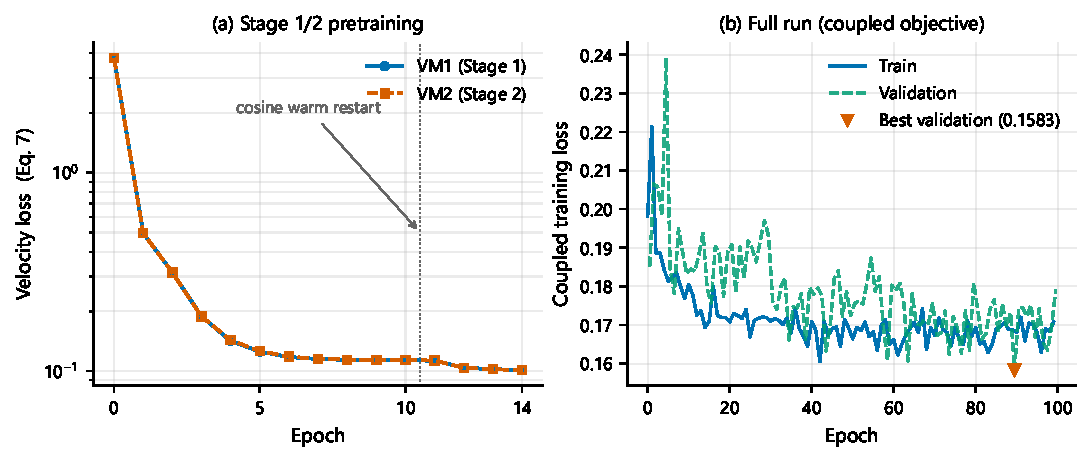
\includegraphics[width=\linewidth]{figures/training_curves.pdf}
  \caption{(a) Stage~1/2 pretraining (Eq.~7 velocity loss, one value per epoch) from the staged rerun of July 2026. The two independent runs are nearly indistinguishable, and the loss falls by a factor of 37 before the cosine warm restart at epoch~11; both settle at ${\approx}0.101$. (b) The full coupled training run of May 2026 that produced the best submission (train and validation loss, one epoch per point). Both curves plateau by epoch ${\sim}40$; the remaining 60 epochs did not improve the metric.}
  \label{fig:curves}
\end{figure}

\subsection{Training dynamics}

The staged pretraining runs are reproducible: VM1 and VM2, trained independently from different seeds with the same recipe, follow nearly identical trajectories, from 3.78 down to 0.101 over 15 epochs. Both the pretraining and the coupled run also reach their loss floors quickly: within 5 and about 40 epochs respectively. The remaining 60 epochs of the coupled run changed neither the loss nor the metric, and Section~\ref{sec:postmortem} argues that what kept the two from falling further was the training target rather than the optimizer.

\subsection{What changed the numbers}

The competition metric improved only through changes made in sequence, and none of them was ablated in isolation; the 67.44 of Table~\ref{tab:glance} came after all of them. Three were followed by better scores. Training on 8 patches of 1{,}000 points per sample instead of one multiplied the supervised points per sample by eight. Moving inference from whole-cloud Euler integration to patch-based filtering removed both a train/inference statistics mismatch and the memory ceiling. Feeding the encoder the same interpolation state used in training when computing the coupled state ($X_{t_1}$) removed a small distribution shift. Two further changes were throughput and stability work rather than accuracy work: removing the distance module from the phase-1 forward pass, which cut encoder calls per step from three to two, and the reconstruction vectorization and sync discipline of Section~\ref{sec:jittor}.

%=============================================================================
\section{Post-Mortem: What Failed and Why}
\label{sec:postmortem}
%=============================================================================

\paragraph{The merged schedule and the distance module.} The paper's staged schedule is not incidental: the distance module is trained last \emph{with the backbone frozen}, so that it learns to scale step sizes against a stationary feature distribution. Our competition schedule instead trained the distance module briefly and then unfroze the backbone, after which the features it had learned against changed.

The July re-tuning changed several things at once: the velocity target, the encoder input state, the addition of the coupling term, the noise schedule, and the number of encoder layers. Its lower score therefore cannot be attributed to any single change. But the regression is confined to one half of the metric: P2S fell from 82.9 to 77.9 while CD was unchanged. A broken velocity field would move both; a broken step-size regulator moves only P2S, which is what we see. We think the distance module is the cause, and we found the evidence after the submission window had closed.

\paragraph{Noise-model drift.} The method's mathematics assumes interpolation between a noisy and a clean sample of the \emph{same} noise family: the velocity target $X_1 - X_0$ is meaningful because $X_t$ moves along that line. The competition's noise is Laplace. We trained with a ``mixed'' schedule (60\% Laplace, 20\% Gaussian, 20\% uniform) intended to hedge, which violates the interpolation assumption for two-fifths of the samples and bought nothing measurable.

The staged rerun measured how much this matters. Scoring is relative to the noisy input, so a score of 1 is as low as a working model can go: a single velocity module pretrained on pure Gaussian noise, its velocity loss down to 0.101, scores 1.01/100 on the competition's Laplace noise, with a CD sub-score of 0.00 and a P2S sub-score of 2.03. Trained on one noise family, the module has nothing to offer the other. The staged reruns kept the paper's Gaussian choice, so that measurement is a sensitivity check rather than a fix. The move we should have made is the one we avoided: train on Laplace, the distribution we would be scored on, rather than hedging inside a framework whose math assumes a specific family.

\paragraph{Inference repetition.} Our inference repeats the patch filter 2--4 times depending on estimated noise. Repeating the filter raises the score, because iterated Euclidean projections onto an imperfectly straight field behave like a curved path, but the reported quality then comes partly from inference compute rather than from the velocity field. Under the paper's single pass we could not reproduce the paper's numbers.

\paragraph{A plateau we did not diagnose in time.} Loss floors at epoch 5 (pretraining) and ${\sim}40$ (coupled) with no metric movement afterward should have redirected us from learning-rate tuning to the objective itself: the loss is a proxy, and nothing guaranteed that driving it to its floor would optimize CD/P2S. The metric harness that could have told us this earlier was itself built mid-competition --- a sequencing mistake.

\paragraph{The score-based detour.} In the final weeks we implemented a ScoreDenoise-style~\citep{scoredenoise} variant reusing the same encoder/decoder: the target becomes the empirical score $\mathrm{NN}(X_t, X_{\text{clean}}) - X_t$ and inference becomes annealed Langevin dynamics. It is distribution-agnostic --- it assumes neither a noise family nor straight paths --- which is the property our Laplace/Gaussian mismatch needed. The implementation hit memory problems on the $O(N^2)$ nearest-neighbour target over 1{,}000-point patches, solved first by chunking and finally by computing targets on the CPU with \texttt{cKDTree}; the code exists in the repository (\texttt{src/model/score\_vm.py}) and was never trained to a comparable state before the deadline. It consumed the last stretch of the competition and produced no scored result.

\paragraph{Process.} Three process failures, in decreasing order of cost: the schedule-faithful rerun started after the submission was frozen rather than before it; the official-metric harness arrived late, so weeks were spent optimizing a proxy loss; and with a single part-time participant, the last-mile work --- running the proper schedule to completion --- did not fit the window.

%=============================================================================
\section{The Qualification Round: PCT for ModelNet40}
\label{sec:warmup}
%=============================================================================

The track opened with a qualification round: classify ModelNet40 shapes from 2{,}048 points into 40 categories, in Jittor, with a test-accuracy threshold of 80\% to advance. Our entry ranked 12th in the round.

\subsection{Model}

The final model follows the full architecture of the PCT paper~\citep{pct} (${\sim}2.9$M parameters): a convolutional stem ($3{\to}64{\to}64$), two sample-and-group stages (farthest-point sampling $1024{\to}512{\to}256$, $k$-NN with $k=32$, local feature aggregation), four offset-attention layers with position encoding and residual connections, a concatenated skip into a $1280{\to}1024$ projection, and a max-pooled classifier ($1024{\to}512{\to}256{\to}40$).

Two details deviate from the reference implementation. The four attention layers each carry their own positional projection rather than sharing one; we have no ablation that isolates the effect of this change. And the low-level operators are hand-written: \texttt{rf\_ops.py} implements farthest-point sampling with a shared-memory reduction, a ported $k$-NN, and index-based point gathering as Jittor CUDA ops.

\subsection{Training recipe, and what actually helped}

Training used AdamW at lr $0.01$ with weight decay $10^{-4}$ and a warmup-cosine schedule over 300 epochs, batch size 32, label smoothing 0.1, dropout 0.5, and weight EMA. The augmentation set scaled the cloud randomly to $[0.67, 1.5]$, translated it by $\pm 0.2$, dropped 10--40\% of the points, and added Gaussian jitter at $\sigma = 0.01$; rotation augmentation appeared in earlier versions and was removed during tuning. Validation used a fixed 90/10 split.

The version history is short. A minimal PCT already cleared the threshold at about 80\% accuracy: four attention layers, no sample-and-group stages, rotation-only augmentation, SGD with cosine annealing. An experiment that added a geometric attention bias, rescaling pairwise Euclidean distances by a learned factor, underperformed and was dropped. What moved the result was the hierarchical sample-and-group stages and the widened augmentation set. Per-version accuracies were not recorded.

The data-side work produced the gains here --- augmentation ranges, the sample-and-group stages, the validation split --- and architecture variants did not. On the main track the emphasis inverted: weeks went into architecture and schedule variants while the noise model and the evaluation harness were fixed late.

\subsection{Dropout that ignores the training flag}

Jittor's dropout layers did not follow the module's training flag reliably in our version. The final training script works around this by walking the module tree and setting every dropout layer explicitly (\texttt{\_set\_dropout\_train}) at the start of each epoch and before validation. Until that fix, runs trained with dropout in an unintended state, and nothing in the loss curves or the logs would have announced it.

%=============================================================================
\section{Lessons Learned}
\label{sec:lessons}
%=============================================================================

\begin{itemize}
  \item \emph{The training schedule is part of the method.} The largest gap to the paper came from a training-order deviation we chose for expedience; when components are trained against each other's frozen states, the order determines what they learn.
  \item \emph{A loss floor is not a metric result.} Both losses reached clean floors and the metric did not follow. The held-out harness for the real metric belonged in the first week.
  \item \emph{Hedging inside a method's assumptions does not pay.} Mixed-noise training cost fidelity to the interpolation premise and bought nothing measurable.
  \item \emph{Inference tricks that compensate hide what is broken.} Repeating the filter raised the score and concealed a velocity field that was not straight enough.
  \item \emph{Memory discipline is part of the model in Jittor.} \texttt{sync\_all}/\texttt{gc} placement, chunked KNN, and patch-batch caps made long runs possible and change what can be trained, not just how fast.
  \item \emph{Look for per-iteration \texttt{.item()} calls first.} They dominated reconstruction until vectorized; the pattern repeated in FPS and KNN.
  \item \emph{MPI data parallelism was cheap; the primitives were not.} Jittor's broadcast/all-reduce integration worked in an afternoon, and the time went to KNN, memory, and the metric.
\end{itemize}

%=============================================================================
\section{Reproducibility}
\label{sec:repro}
%=============================================================================

The repository contains the training and evaluation pipeline. Training and inference run through \texttt{denoise/run.py} with per-task YAML configs under \texttt{denoise/configs/}: \texttt{train\_vm.yaml} (the merged schedule that produced the submission), \texttt{train\_vm\_stage\{1..4\}.yaml} (the paper's schedule), \texttt{predict\_vm.yaml}, and \texttt{train\_score.yaml} (the untrained score-based variant). Evaluation is \texttt{self\_eval.py} (held-out split, full metric) and \texttt{evaluate.py} (official-style scoring); diagnostics are \texttt{profile.py} and \texttt{vis\_denoising.py}. Figures and tables in this report are generated by \texttt{report/make\_figures.py} from the run logs (the May run log is included under \texttt{report/data/}). The dataset --- ShapeNet meshes and the pre-noised test clouds --- is provided by the competition organizers and is not redistributed here; datalist files define the splits.

\vspace{0.8em}
\noindent\rule{\linewidth}{0.4pt}
\vspace{-0.4em}
\begin{quote}
\small \emph{Acknowledgement of scope.} The task definition, dataset, and evaluation protocol belong to the organizers of the 6th Jittor AI Challenge (Track~2). The StraightPCF method and its equations are due to \citet{straightpcf}. The implementation in Jittor, the experiments, the evaluation harness, and all measurements and errors in this report are my own.
\end{quote}

\begin{thebibliography}{9}

\bibitem[de Silva Edirimuni et al.(2024)]{straightpcf}
Dasith de Silva Edirimuni, Xuequan Lu, Gang Li, Lei Wei, Antonio Robles-Kelly, and Hongdong Li.
\newblock StraightPCF: Straight point cloud filtering.
\newblock In \emph{Proceedings of the IEEE/CVF Conference on Computer Vision and Pattern Recognition (CVPR)}, 2024.

\bibitem[Luo and Hu(2021)]{scoredenoise}
Shitong Luo and Wei Hu.
\newblock Score-based point cloud denoising.
\newblock In \emph{Proceedings of the IEEE/CVF International Conference on Computer Vision (ICCV)}, 2021.

\bibitem[Guo et al.(2021)]{pct}
Meng-Hao Guo, Jun-Xiong Cai, Zheng-Ning Liu, Tai-Jiang Mu, Ralph R. Martin, and Shi-Min Hu.
\newblock PCT: Point cloud transformer.
\newblock \emph{Computational Visual Media}, 7(2):187--199, 2021.

\bibitem[Qi et al.(2017)]{pointnet}
Charles R. Qi, Hao Su, Kaichun Mo, and Leonidas J. Guibas.
\newblock PointNet: Deep learning on point sets for 3D classification and segmentation.
\newblock In \emph{CVPR}, 2017.

\end{thebibliography}

\end{document}
